\documentclass[a4paper,11pt]{article}
\pdfoutput=1 % if your are submitting a pdflatex (i.e. if you have
             % images in pdf, png or jpg format)
\usepackage{color}
\usepackage{jcappub} % for details on the use of the package, please
                     %
\usepackage{amsmath}
\newcommand\ddfrac[2]{\frac{\displaystyle #1}{\displaystyle #2}}

\usepackage[T1]{fontenc} % if needed
\usepackage{threeparttable}
\usepackage[labelformat=empty]{subfig}
\usepackage{booktabs}
\usepackage{multirow}
\usepackage{placeins}
\usepackage[utf8]{inputenc}
\usepackage{indentfirst}
\usepackage[utf8]{inputenc}

\title{\boldmath Flux Conventions in the Neutrino Sources Group}

\author[a]{Alex Pizzuto,}
\author[a]{Justin Vandenbroucke}


\affiliation[a]{Dept. of Physics and Wisconsin IceCube Particle Astrophysics Center, University of Wisconsin, Madison, WI 53706, USA }

\emailAdd{apizzuto@icecube.wisc.edu}

\abstract{}

\notoc %this turns off the table of contents
\begin{document} 
\maketitle
\flushbottom

% \section{Introduction\label{sec:intro}}
% One of the predominant scientific goals of IceCube is the detection of astrophysical neutrino sources. To this end, BLA BLA MAXIMUM LIKELIHOOD REFERENCE. Fortunately, we seem to be in the era when individual sources of astrophysical neutrinos are becoming detectable above our atmospheric backgrounds. However, this UNDERSCORES the importance of clear and consistent notation. As the hypotheses which we test in the neutrino sources WG can vary greatly, 

% \section{Flux vs. Fluence}
% Suppose we have a source of astrophysical neutrinos that produces a flux at Earth at the level of

% \begin{equation}
%     \frac{dN}{dEdAdt} = \phi_0 \Big(\frac{E}{E_0}\Big)^{-\gamma}\;,
% \end{equation}
% where $\phi_0$ is a normalization that carries units GeV$^{-1}$~cm$^{-2}$~s$^{-1}$.

% \begin{tabular}{l|c|c}
%      &  \\
%      & 
% \end{tabular}

% \section{Unbroken power laws}
% Mention why E-2 are convenient (you don't need a reference energy). but this leads to confusion because without mention of a reference energy you might think that it's an integrated quantity

\section{Energy Ranges for sensitivities}
\label{sec:energy_range}
One crucial ingredient needed for constraining astrophysical neutrino production is the energy range at which an upper limit -- or a measurement -- is valid. We know that IceCube is sensitive in roughly the TeV -- PeV range, but the exact energies which are most important in a source search are dependent on the event selection, source direction, and assumed spectral shape.

The most descriptive way to quantify the sensitive energy range is by calculating a full differential sensitivity (see \href{https://internal-apps.icecube.wisc.edu/reports/details.php?type=report&id=icecube\%2F201910002}{Rene's internal note} on how to do this in a computationally feasible way). However, it is also informative to constrain benchmark models, such as simple power laws, where the flux is defined as 

\begin{equation}
     \frac{dN}{dEdAdT} \equiv \phi(E) = \phi_0 \Big(\frac{E}{E_0}\Big)^{-\gamma} \; .
\end{equation}

While the PDF of this flux has support on $(0, \infty)$, our detector is not sensitive over all energies. Note that for the purposes of this note we interchangeably use the notation $dN\big/dEdAdT$ and $\phi(E)$ to represent the energy-differential point source flux, which carries units GeV$^{-1}$~cm$^{-1}$~s$^{-1}$. We will use the former when trying to be explicit about the units and the latter for shorthand. To calculate the energy range to which an analysis is sensitive at a specified CL ($\alpha$), there are a couple of accepted methods used in the working group:

\begin{itemize}
    \item \textbf{Method 1 (Effective area construction):} Calculate the central energy range that contains the fraction $\alpha$ of signal events when injecting the assumed spectral shape
    \item \textbf{Method 2 (Sensitivity construction):} Remove the lowest energy events from simulated signal until the sensitivity degrades by a factor $(1-\alpha)/2$. Repeat for the highest energy events.
\end{itemize}

It is worth noting that these are only for calculating projected sensitivities. When looking at the energy range which is most important in a specific measurement, there are other methods (\href{https://drive.google.com/file/d/1UVBMbMJwyqDicMsBtyAmF3kLzf-pcnSS/view}{see Christian Haack's talk in nu-sources}). Below, we discuss the specifics of these two methods, and discuss in what regimes the two methods are equivalent.

\textbf{Effective area construction.} The effective area construction answers the question ``what is the range of true neutrino energies that will be present in the data under the given assumed spectral hypothesis?'' The goal of this construction is to calculate two threshold energies, $E_{\mathrm{min}}$ and $E_{\mathrm{max}}$, such that 

\begin{equation}
    \frac{\displaystyle\int_{0}^{E_{\mathrm{min}}}\phi(E) A_{\mathrm{eff}}(E, \delta)\; dE}{\displaystyle\int_{0}^{\infty}\phi(E) A_{\mathrm{eff}}(E, \delta)\; dE}  = \frac{1-\alpha}{2} \quad \& \quad \frac{\displaystyle\int_{0}^{E_{\mathrm{max}}}\phi(E) A_{\mathrm{eff}}(E, \delta)\; dE}{\displaystyle\int_{0}^{\infty}\phi(E) A_{\mathrm{eff}}(E, \delta)\; dE}  = \frac{1+\alpha}{2} \, .
\end{equation}

\begin{figure}
    \centering
    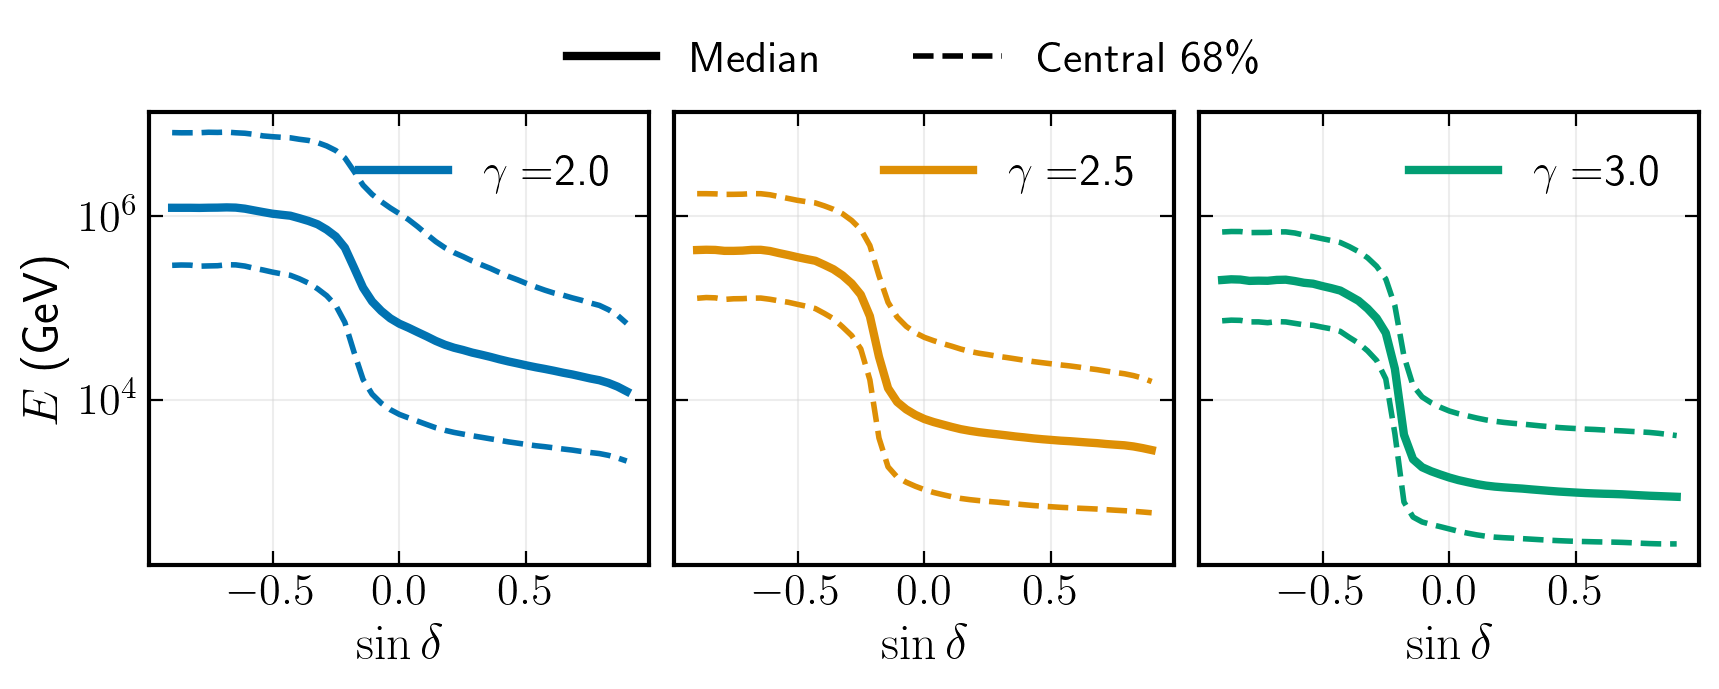
\includegraphics[width=0.95\textwidth]{figures/gfu_central_energies_effective_area.png}
    \caption{Central 68\% energy range calculated with the effective area construction for the GFU sample as a function of declination, for a variety of spectral indices.}
    \label{fig:central_en_eff_area_gfu}
\end{figure}

This is equivalent to weighting a Monte Carlo sample of events by the assumed spectral shape and calculating the CDF of the true neutrino energies. Finding where this CDF is equal to $\frac{1\mp\alpha}{2}$ will yield the relevant threshold energies. Figure~\ref{fig:central_en_eff_area_gfu} displays these energy ranges with $\alpha=0.68$ using the GFU sample (\texttt{GFUv002p05}). The central energy ranges calculated with a different event selection would of course differ, but they should be similar for other high-statistics track-based selections. This method has the advantage of a small computation time. 

\textbf{Sensitivity Construction.} The sensitivity construction answers a similar, albeit slightly different, question when compared to the effective area construction. This construction answers the question ``for a given assumed spectral hypothesis, which energies contribute most to the sensitivity of the analysis?'' To calculate this range, first find the sensitivity flux using the standard procedure, call this value $\phi_{\mathrm{sens}}$. Then, repeat the calculation, but when initializing the analysis introduce a threshold, $E_{\mathrm{cut}}$ and exclude all signal events where $E_{\nu, \mathrm{true}} < E_{\mathrm{cut}}$. Float the threshold energy until the flux needed for sensitivity is $\frac{2\phi_{\mathrm{sens}}}{1+\alpha}$. Figure~\ref{fig:central_en_sensitivity_gfu} shows how this was calculated for a sample single point source analysis. This method is significantly more computationally intensive, as it requires the analyzer to recalculate the sensitivity of the analysis for a multitude of allowable $E_{\mathrm{cut}}$ values. 

\begin{figure}
    \centering
    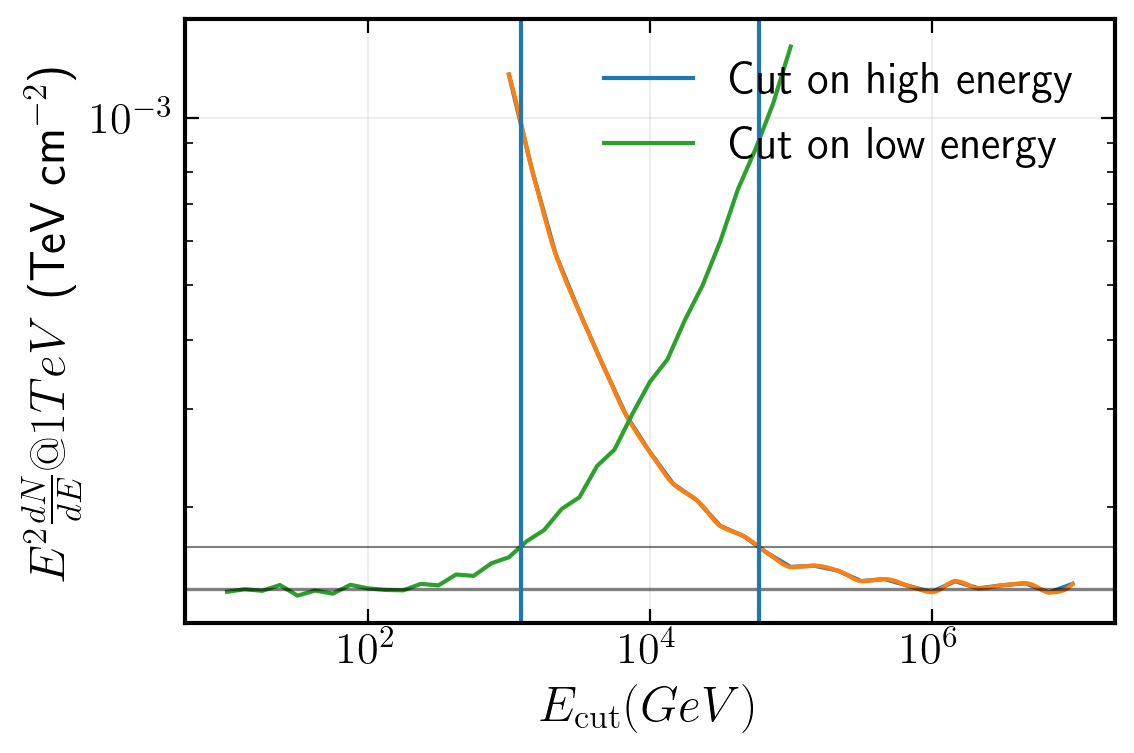
\includegraphics[width=0.5\textwidth]{figures/sensitivity_en_range_gfu.png}
    \caption{Sensitivity for a single source at $\delta=0^{\circ}$, with an analysis time window of $10^5$ s and an injected spectral index of $\gamma=2.5$. The lower and higher horizontal lines show $\phi_{\mathrm{sens}}$ and  $\frac{2\phi_{\mathrm{sens}}}{1+\alpha}$, respectively, with $\alpha=0.68$. The threshold energies are shown with vertical lines.}
    \label{fig:central_en_sensitivity_gfu}
\end{figure}

These methods are similar in motivation, but for large background analyses the energy ranges which we calculate can differ. However, for short timescales, the methods are equivalent. This is because at short timescales, our likelihood analyses function as counting experiments, and any signal event will yield a significant result. In this regime, the only thing that will affect the sensitivity is the detector response, meaning that the sensitivity will scale inversely and linearly with the effective area. Finding where the sensitivity degrades by a fraction of $\frac{1-\alpha}{2}$ is then the same as asking where the effective area is reduced by the same factor.

\begin{figure}
    \centering
    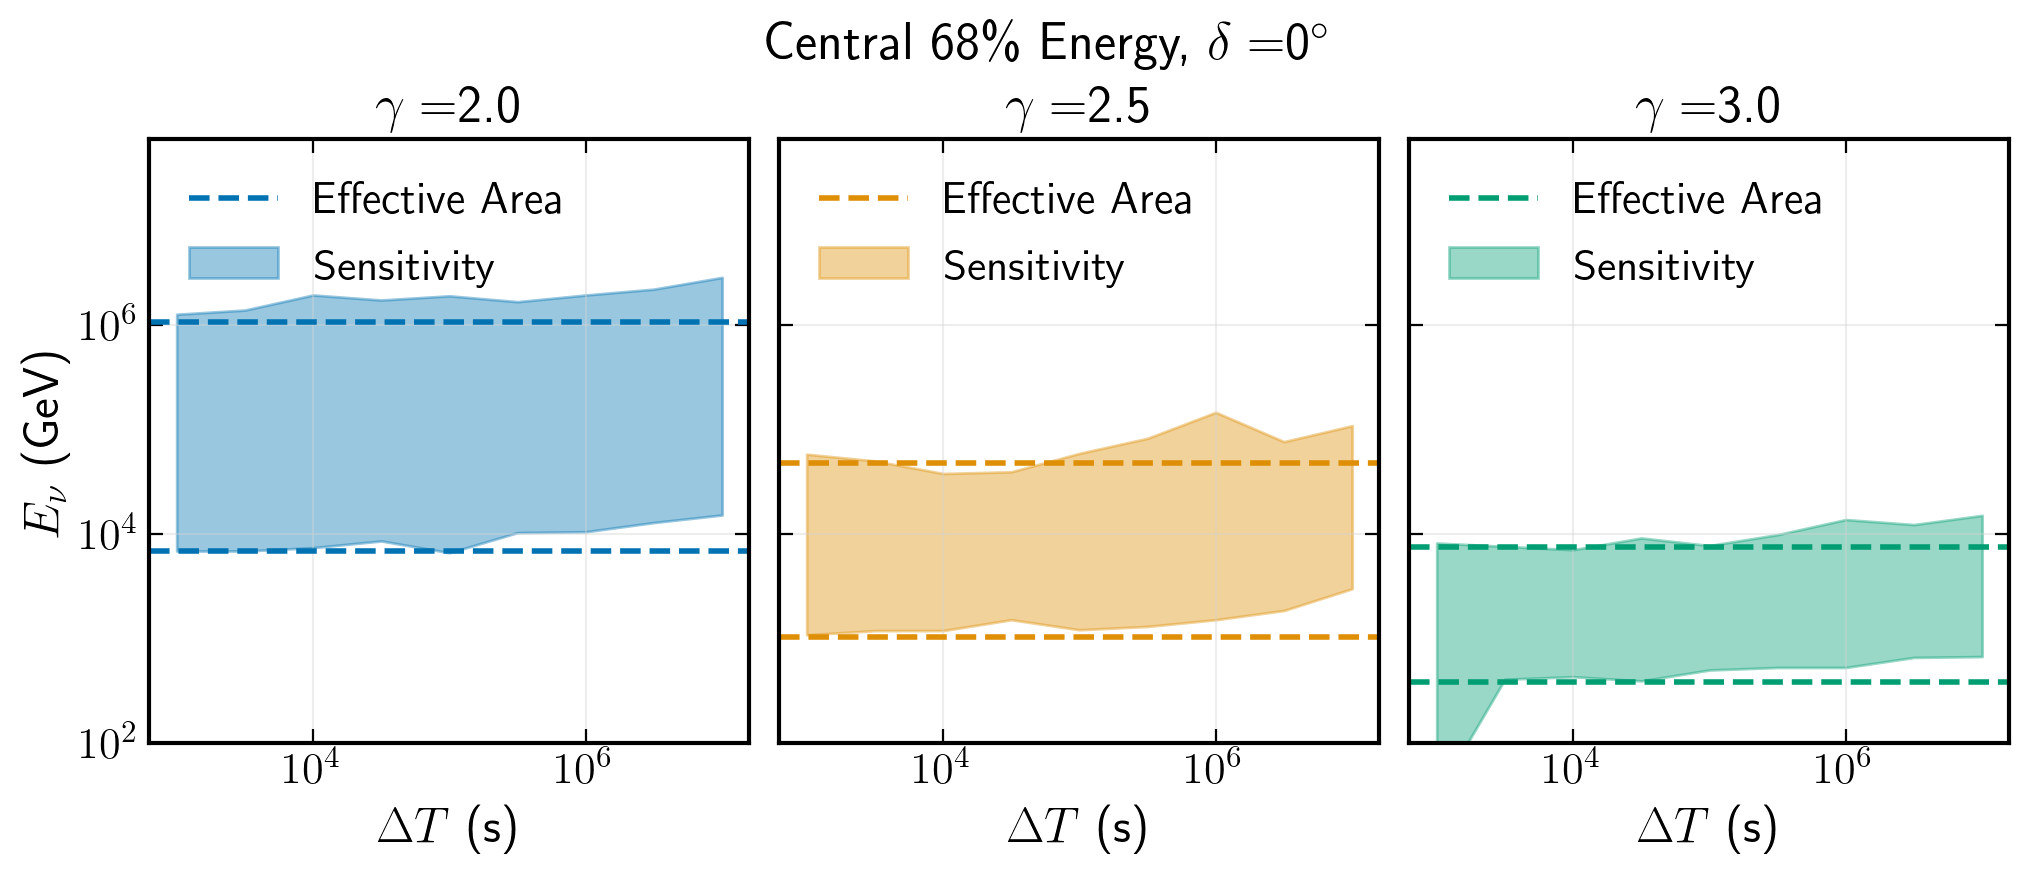
\includegraphics[width=0.98\textwidth]{figures/central_en_comparison_gfu.png}
    \caption{Central energy ranges under the ``effective area'' construction (dashed) and the ``sensitivity'' construction (shaded) for three different spectral indices. For short timescale analyses, the methods are equivalent, but diverge for larger time windows where the sensitivity construction will shift towards higher energy events.}
    \label{fig:energy_range_comparison}
\end{figure}

Figure~\ref{fig:energy_range_comparison} shows this comparison explicitly, for a source at the horizon. This Figure highlights that for small background (short timescale) analyses, the two constructions are equivalent. However, for larger time windows, the extra per-event information becomes important, and the energy range which contributes to the sensitivity shifts towards higher energies, where events on average are better reconstructed and are easier to distinguish from background. For this reason, we recommend the analyzer use the ``effective area'' construction for short timescale (ie low-background) analyses, to reduce the computational requirements. For longer timescales, it is up to the analyzer to decide which question is more prudent for their analysis. It is worth noting that all of the examples in the Figures above set $\alpha=0.68$ in order to minimize the statistics needed in calculating various sensitivities, though all of the same logic holds for the more common convention of $\alpha=0.90$. 

\section{Flux Nomenclature}
Arguably, just as important as the energy range at which an analysis is most sensitive is the magnitude that such as flux needs in order to for an analysis to be sensitive to it. For analyses that test non-steady temporal hypothesis (eg. ``transient'' analyses or ``flare'' analyses), there is the added confusion of describing this flux succinctly even though it changes as a function of time. To get around this problem, we often describe fluxes in terms of time-integrated quantities, ie in terms of a ``fluence''. There are a few different conventions -- all of which correspond to slightly different physical quantities -- which we outline below.

\begin{enumerate}
    \item Time-integrated differential energy flux, $\mathcal{F}$ (``particle fluence''):
    \begin{equation}
        \mathcal{F}(E) = \int \frac{dN}{dEdAdT} dT
    \end{equation}
    \item ``Energy fluence,'' $\mathbb{F}(E_a, E_b)$:
    \begin{equation}
        \mathbb{F}(E_a, E_b) = \int\int_{E_a}^{E_b} E \frac{dN}{dEdAdT} dEdT
    \end{equation}
\end{enumerate}

Physically, these different fluences refer to two distinct quantities, as indicated by their names. The ``particle fluence,'' $\mathcal{F}(E)$, quantifies the \textit{number of particles of a certain energy that pass through an area in a given time}. The ``energy fluence,'' $\mathbb{F}(E_a, E_b)$, is the \textit{amount of energy in a flux per unit area in a given time over a specific energy interval}.

MENTION PAGE 3 FROM GAISSER AND RESCONI

When quoting sensitivities, we often do this in terms of the particle fluence, $\mathcal{F}(E)$, scaled by a factor of energy-squared, $E^2\mathcal{F}(E)$ (in much of our internal software, such as \texttt{csky}, this quantity is called $E^2dN/dE$). Scaling a flux by $E^2$ has a variety of benefits -- it serves as a proxy for the energy content in a flux, when showing the flux over many orders of magnitudes subtle changes in slope become more apparent, and for the special case of the prototypical $E^{-2}$ this quantity is independent of energy.

However, this energy scaling results in a confusion between these two quantities, as

\begin{equation}
    \big[E^2\mathcal{F}(E)\big] = \big[\mathbb{F}(E_a, E_b)\big] = \mathrm{GeV}\;\mathrm{cm}^{-2}\;,
\end{equation}
and also because in some papers we have a tendency to just quote the ``fluence'' needed for sensitivity instead of clarifying if this ``fluence'' is an energy fluence or energy-squared times particle fluence. This leads to confusion when we just quote ``a fluence of $x$ GeV cm$^{-2}$,'' which at face value seems like an energy fluence as it is not clear over what energy range this is applicable. However, we are usually discussing a particle fluence at a particular energy, which is not clear because we do not specify that we have scaled a particle fluence by $E^2$ to have these units.

Although we normally discuss particle fluences for sensitivities, we still often want to calculate the energy in a flux, for which we need to specify an energy interval. For calculating the energy interval, we often use the methods outlined in Section~\ref{sec:energy_range}.
\newline
\textbf{Example: Power-laws}

Suppose we have an astrophysical source which emits neutrinos according to a power-law spectrum, 
\begin{equation}
    \frac{dN}{dEdAdT}= \phi_0 \Big(\frac{E}{E_0}\Big)^{-\gamma} \; ,
\end{equation}
and we collect data on this source for an observation period of $\Delta T$. The energy-scaled time-integrated differential energy flux and the energy fluence are calculated as 

\begin{equation*}
\begin{aligned}[c]
    E^2\mathcal{F}(E) &= E^2\int \frac{dN}{dEdAdT} dT \\
    &= E^2 \Delta T \phi_0 \Big(\frac{E}{E_0}\Big)^{-\gamma} \\
    &= \phi_0 E_0^{\gamma} E^{2-\gamma}\Delta T
\end{aligned}
\qquad\&\qquad
\begin{aligned}[c]
    \mathbb{F}(E_a, E_b) &= \int dT \int_{E_a}^{E_b} E \frac{dN}{dEdAdT} dE \\ 
    &= \Delta T \int_{E_a}^{E_b} E \phi_0 \Big(\frac{E}{E_0}\Big)^{-\gamma} dE \\
    &= \phi_0 \Delta T E_0^{\gamma} \times \begin{cases}
            \ddfrac{E^{1-\gamma}}{1-\gamma}\Big|_{E_a}^{E_b} &\gamma\neq 2 \\ \log\big(\ddfrac{E_b}{E_a}\big) & \gamma = 2
        \end{cases}
\end{aligned}
\end{equation*}

In the case of $\gamma = 2$, we have 
\begin{equation}
    \frac{\mathbb{F}(E_a, E_b)}{E^2\mathcal{F}(E)} = \log\big(\ddfrac{E_b}{E_a}\big) \; ,
\end{equation}
so in the case of an $E^{-2}$, where the energy output per decade in energy is a constant, then we can interpret $E^2\mathcal{F}(E)$ as the energy fluence per logarithmic energy interval.

For all other spectral indices, we have
\begin{equation}
    \frac{\mathbb{F}(E_a, E_b)}{E^2\mathcal{F}(E)} = 
    \frac{1}{1-\gamma}\frac{E_b^{1-\gamma} - E_a^{1-\gamma}}{E^{2-\gamma}} \; ,
\end{equation}
and it is clear that we are not as able to draw immediate parallels between these two physical quantities.

It is also worth noting that in order to convert a flux to the amount of energy that an astrophysical source emits (or its luminosity for constant fluxes), one must properly take into account cosmic expansion and how this affects (1) the duration of a transient and (2) the energy of the particles emitted. For this entire discussion, we are assuming all times are in the observer frame. For more discussion on the differences between fluxes and fluences and between energy and particle fluxes, and specifically how they behave differently due to cosmic expansions, I would strongly recommend reading Appendix B of Nora Linn Strojohann's thesis \cite{norathesis}.

Moving forwards, we would like to advocate that all fluxes are which are quoted are defined explicitly in\footnote{This is a pain in the butt because sometimes in theory / model papers the fluence is used interchangeably to describe these two quantities?LIST OF PAPER WHERE THIS IS DONE WITH DIFFERENT WAYS}

\section{Differential Sensitivity}
Look at Rene's internal note for a lot of this, and cite it

\section{Bin width problem}
Differential sensitivity is a function of the bin-width?

\subsection{Comparing to Models and Model Rejection Factors}
Because our differential sensitivity is a function of bin-width, show fluxes we are / aren't sensitive to

% \section{Constraining physics quantities: Energies, luminosities, etc.}
% Maybe mention the need to correct for redshift? Look at Nora's thesis

% \section{Time-dependent fluxes}

% Fluence:

% \begin{align}
%     \iint E \frac{dN}{dEdAdT} dE dT &= \Delta T \int_{\{E\}} E \phi_0 \Big(\frac{E}{E_0}\Big)^{-\gamma} dE \\
%     &= \phi_0 \Delta T E_0^{\gamma} \int_{\{E\}} E^{-\gamma + 1} dE \\ 
%     &= 
% \end{align}
% with units $[ \mathcal{F}] = $GeV$\cdot$cm$^{-2}$.

% \begin{align}
%     E^2 \int \frac{dN}{dEdAdT} dT &= E^2 \Delta T \phi_0 \Big(\frac{E}{E_0}\Big)^{-2} \\
%     &= \phi_0 E_0^2 \Delta T 
% \end{align}

Takeaways:
\begin{itemize}
    \item When calculating an energy range, bla
    \item Always define your fluxes and sensitivities in terms of what they represent differentially, before calling something a ``fluence.'' If you want to use the word fluence, be explicit about wheter this is a particle fluence or energy fluence
    \item Often the central 90\% energy interval does not capture the entire energy dependence of an analysis, in order to do this, calculate a differential sensitivity
    \item Be cautious of interpreting differential sensitivities
\end{itemize}

\bibliographystyle{JHEP}
\bibliography{references}

\end{document}
